\documentclass{beamer}
\usepackage[russian]{babel}
\usetheme{metropolis}

\usepackage{amsthm}
\setbeamertemplate{theorems}[numbered]

\setbeamercolor{block title}{use=structure,fg=white,bg=gray!75!black}
\setbeamercolor{block body}{use=structure,fg=black,bg=gray!20!white}

\usepackage[T2A]{fontenc}
\usepackage[utf8]{inputenc}

\usepackage{hyphenat}
\usepackage{amsmath}
\usepackage{graphicx}

\AtBeginEnvironment{proof}{\renewcommand{\qedsymbol}{}}{}{}

\title{
Микроэкономика-I
}
\author{
Павел Андреянов, PhD
}

\begin{document}

\maketitle

\section{Начала оптимизации}

\begin{frame}{Начала оптимизации}

Любая оптимизационная задача это две вещи
- функция, которую мы максимизируем
- область определения аргументов, по которым мы максимизируем

Ключевыми факторами тут являются непрерывность целевой функции и выпуклость области определения.

\end{frame}

\section{Непрерывность}

\begin{frame}{Непрерывность}

Существование решения, как правило, мы можем легко гарантировать при помощи следующей теоремы

\begin{theorem}[Вейерштрасса]

Непрерывная функция на компакте гарантированно достигает своего минимума и максимума.
\end{theorem}

Что такое непрерывная функция вы уже знаете.

\end{frame}

\begin{frame}{Непрерывность}

A \textbf{компакт} в $\mathbb{R}^n$ это просто ограниченное и замкнутое множество. 

В контексте одномерной оптимизации, $[a,b]$ это компакт, а $(a,b]$, $[a,b)$, $(a,b)$, $[a,\infty)$,$(a,\infty)$ это все не компакты. 

\end{frame}

\begin{frame}{Непрерывность}

Таким образом, у вас есть всего два сценария как решение оптимизационной задачи с непрерывной функцией могло бы не существовать: либо оно вообще бесконечно, либо оно конечно, но достигается в точке которая попала на границу области.

\end{frame}

\section{Условия Первого Порядка}

\begin{frame}{УПП}

Если решение лежит внутри области, то обязательно выполнены условия первого порядка. Например, если функция $U(x, y, z)$ от трех переменных, и вы убедили себя что решение надо искать внутри, то
$$\text{УПП (FOC)}: \quad  \nabla U = 0$$ 
должны выполняться в оптимальной точке $(x^{\ast}, y^{\ast}, z^{\ast})$. Зачастую, граничных точек не так уж и много, и их можно просто перебрать руками, сравнивая значения. Затем можно выбрать наилучшую из граничных и внутренних точек, удовлетворяющих УПП.

\end{frame}

\begin{frame}{УВП}

Иногда число кандидатов на оптимум, прошедших условия первого порядка,  можно дополнительно сузить за счет условий второго порядка.
$$\text{УВП (SOC)}: \quad  \nabla^2 U \ ? \ 0$$
Если Гессиан во внутренней точке отрицательно определен $\nabla^2 U \leqslant 0$ (парабола рогами вниз) то это локальный максимум и этот кандидат проходит отбор. 

Если Гессиан положительно определен $\nabla^2 U \geqslant 0$ (парабола рогами вверх) то это локальный минимум и этот кандидат не проходит отбор.

\end{frame}

\begin{frame}{УВП}

Если у вас остался один кандидат то он и является оптимумом. 

Если кандидатов несколько то надо опять сравнивать значения функции руками.

\end{frame}

\section{Выпуклость}

\begin{frame}{Выпуклость}

К счастью, в экономике, зачастую удается показать что, поверх непрерывности, функция полезности

\begin{itemize}
\item либо вогнутая
\item либо она монотонное преобразование вогнутой
\item либо она квази-вогнутая
\end{itemize}

Если, вдобавок к этому, область определения не только компакт но и выпуклое множество, то, во первых, решение всегда единственное, а во вторых, условия второго порядка можно не проверять, поскольку они (или что то очень похожее на них) выполнены глобально.

\end{frame}

\begin{frame}{Выпуклость}

Очень важно уметь, глядя на задачу, определять выпуклая она или нет, чтобы не тратить время на анализ второго порядка. 

Общий алгоритм решения выпуклых и непрерывных задач на компакте очень простой:

\begin{itemize}
\item ищем решение как будто оно внутреннее
\item если оно оказалось не внутреннее - ищем на границе
\end{itemize}

В выпуклых задачах условия второго порядка не нужны.

\end{frame}

\section{Линии уровня}

\begin{frame}{Линии уровня}

Наконец, линии уровня это очень удобный инструмент для отлова и классификации кандидатов на решение оптимизационной задачи.

\begin{definition}
\textbf{Линией уровня} полезности $U$, проходящей через точку $x$ называется множество всех точек $y \in X$ таких что $U(y) = U(x)$.
\end{definition}

И есть очень похожее определение для предпочтений...

\end{frame}

\begin{frame}{Кривые безразличия}

\begin{definition}
\textbf{Кривой безразличия} предпочтений $\succcurlyeq$, проходящей через точку $x$ называется множество всех точек $y \in X$ таких что $x \sim y$.
\end{definition}

Совершенно ясно, что в контексте представлений предпочтений полезностями, кривая безразличия и линия уровня это одно и то же.

\end{frame}

\begin{frame}{Линейная полезность}

Рассмотрим полезность вида: $U(x, y) = ax + by$. Тогда линия уровня ищется следующим образом: 
\begin{gather*}
c = ax + by\\
c-ax = by\\
y = \frac{c-ax}{b}
\end{gather*}
Линия уровня это прямая вида $y = \alpha x + \beta$.

\end{frame}

\begin{frame}{Гиперболическая полезность}

Рассмотрим полезность вида: $U(x, y) = a \log x + \log y$. Тогда линия уровня ищется следующим образом: 
\begin{gather*}
c =  a \log x + \log y\\
e^{c} = x^a y\\
y =\frac{e^{c}}{x^a}
\end{gather*}
Линия уровня это гипербола вида $y = x^\alpha \beta$.

\end{frame}

\begin{frame}{Полезность минимум}

Рассмотрим полезность вида: $U(x, y) = \min(ax, by)$. Тогда линия уровня ищется следующим образом: 
\begin{gather*}
c = \min(ax, by)\\
\frac{c}{b}= \min(\frac{a}{b}x, y), \quad \frac{c}{a}= \min(x, \frac{b}{a}y)\\
y = \frac{c}{b} \mathbb{I}(ax > c), \quad x = \frac{c}{a} \mathbb{I}(by > c)
\end{gather*}
Линия уровня это конкатенация горизонтальной и вертикальной линий, соединенных вдоль $ax = by$.

\end{frame}

\begin{frame}{Зачем нужны линии уровня}

Очень часто, в задачах есть выпуклое ограничение типа неравенства, например, бюджетное ограничение. В таком случае, все кандидаты будут формально не внутренние. 

Однако, с точки зрения выпуклой оптимизации, такие точки можно интерпретировать как <<внутренние>>, если решать методом Лагранжа. О методе Лагранжа мы поговорим на следующей лекции.

Внутреннее решение выпуклой (и гладкой) оптимизационной задачи можно охарактеризовать как точку касания линии уровня с выпуклым ограничением.

\end{frame}

\begin{frame}{Квази вогнутость}

\begin{figure}[hbt]
\centering
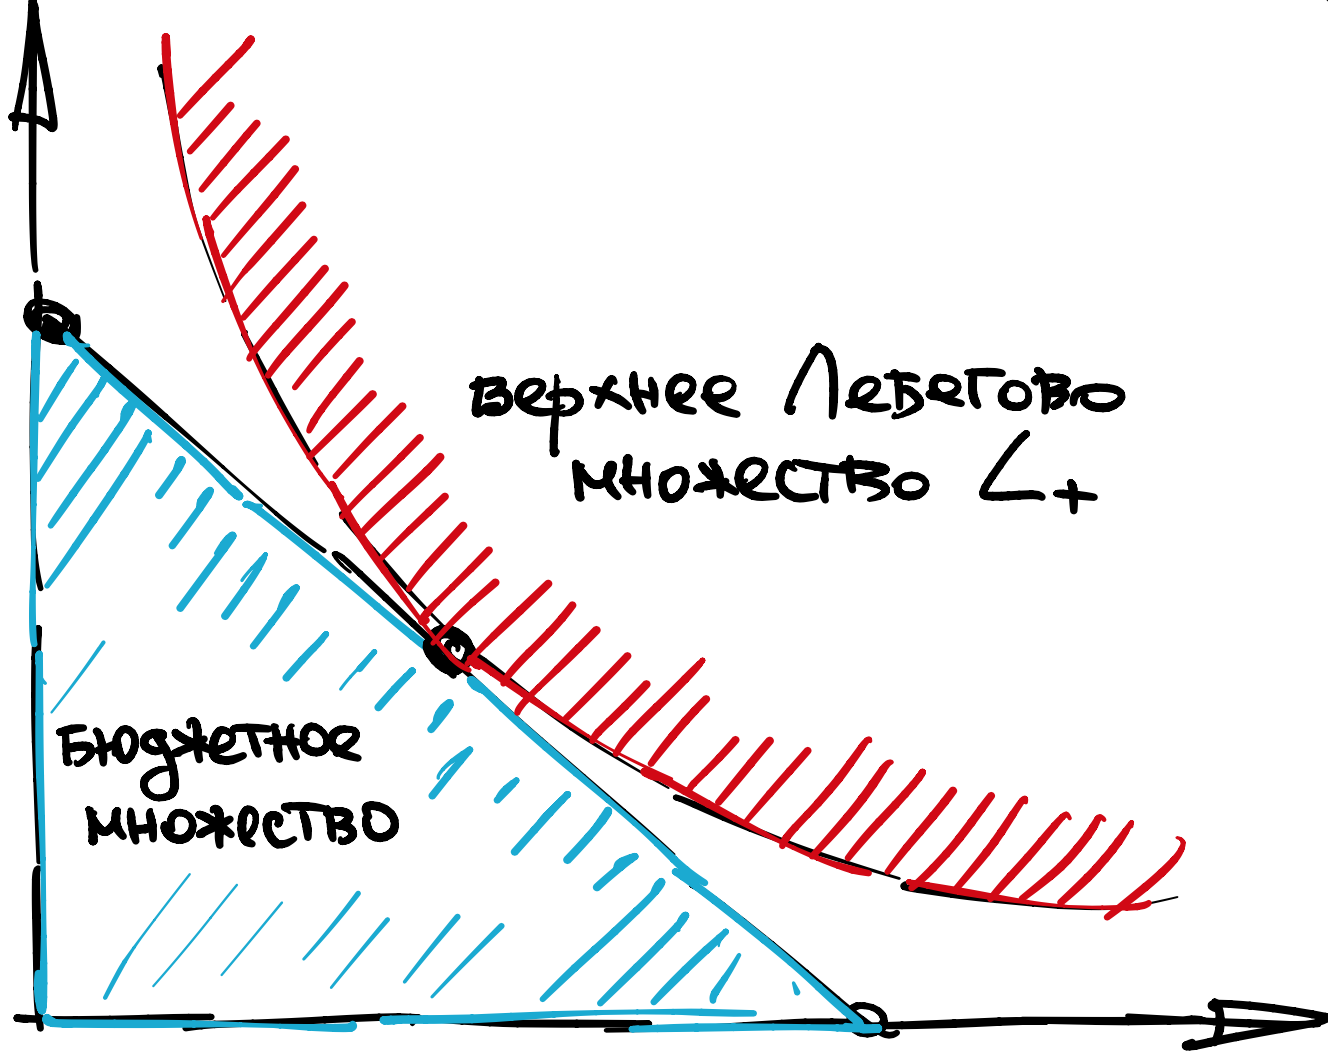
\includegraphics[width=.8 \textwidth]{tangency.png}
\end{figure}

\end{frame}

\section{Конец}

\end{document}